\documentclass[12pt]{article}
\usepackage{../../template}
\title{Lecture 2}
\author{niceguy}
\begin{document}
\maketitle

\section{Parallel Plate Transmission Lines}

We have shown that a parallel plate transmission line can be expressed as the following equivalent circuit.

\begin{figure}[h!]
    \begin{center}
        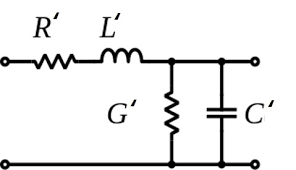
\includegraphics[scale=0.25]{Untitled.png}
    \end{center}
\end{figure}

Using KCL,

$$i(z,t) - i(z+\Delta z,t) = C'\Delta z \del{v(z+\Delta z, t)}{t} + G'\Delta z v(z+\Delta z, t)$$
Dividing by $\Delta z$ and taking the limit as it tends to zero,
$$-\del{i}{t} = C'\del{v}{t} + G'v$$

Similarly, for KVL,

$$-v(z,t) + i(z,t)R'\Delta z + L'\Delta z \del{i(z,t)}{t} + v(z+\Delta z, t) = 0$$
and we get
$$\del{u}{z} = -L'\del{i}{t} - R'i$$

We solve this using phasors. Since we "inject" frequencies at the source, we can safely assume voltage and current are sinusoidal, with the same frequency. For
\begin{align*}
    v(z,t) &= V_0\cos(\omega t + \phi) \\
           &= \Re\{V_0e^{j(\omega t + \phi)}\} \\
           &= \Re\{V_0e^{j\phi}e^{j\omega t}\} \\
           &= \Re\{\tilde V(z)e^{j\omega t}\}
\end{align*}

and similarly
$$i(z,t) = \Re\{\tilde I(z)e^{j\omega t}\}$$
We have now separated space- and time-dependent terms.

this eventually gives
$$\del{\tilde I}{z} = -(G' + j\omega C')\tilde V$$
$$\del{\tilde V}{z} = -(R' + jwL')\tilde I$$

Combining,
\begin{align*}
    \del{^2\tilde V}{z^2} &= -(R' + jwL')\del{\tilde I}{z} \\
                          &= (R' + jwL')(G' + jwC')\tilde V \\
                          &= \gamma^2 \tilde V
\end{align*}

where $\gamma$ is as defined. It is a complex constant, with a real attenuation constant and imaginary phase constant. \\

Then the solution is
$$\tilde V(z) = V_0^+ e^{-\gamma z} + V_0^- e^{\gamma z}$$
and same for $\tilde I(z)$. \\
For a lossless transmission line, $R' = 0$, so
$$\gamma = j\omega\sqrt{L'C'}$$

\end{document}
